\subsection{Kubernetes for NFV}
	
\begin{flushleft}
Kubernetes is a relatively new introduction to the NFV world. The network functions that are made to run in a container are referred to as Containerized Network Functions (CNFs). The CNCF (Cloud Native Computing Federation) is constantly striving to enable Kubernetes as an alternative technology to realize NFV Infrastructure.
\end{flushleft}

\begin{figure}
    \centering
    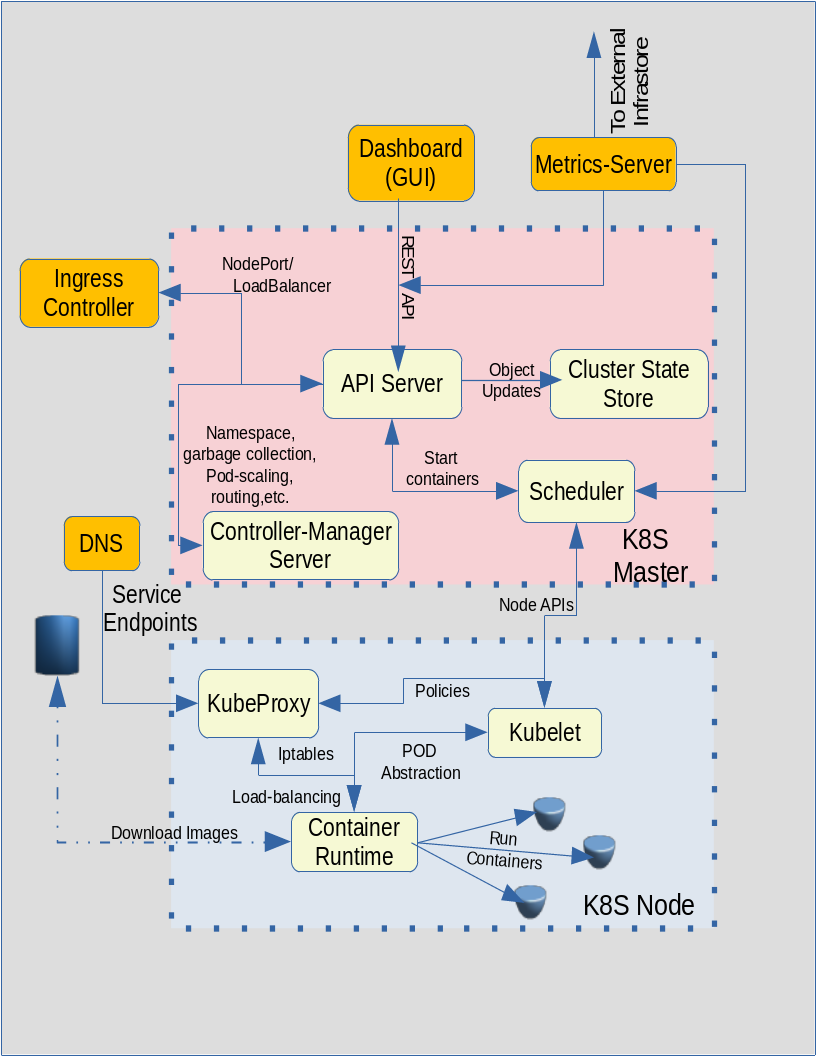
\includegraphics[width=0.5\textwidth]{kubernetes_arch}
    \label{fig:figure16}
    \caption{A block diagram representation of Kubernetes components. Derived from the description in \cite{k8sarch}}
\end{figure}

